\documentclass{beamer}
\usepackage[T1]{fontenc}
\usepackage[utf8]{inputenc}
\usepackage{lmodern}
\usepackage[brazil]{babel}

\usetheme{JuanLesPins}

\title{
       \textbf{Como podemos e devemos monitorar nosso código-fonte} \\
       CCSL - IME - USP
      }
\author{
        Alessandro Palmeira \\
        Daniel Alves \\
        Diego Araújo \\
        Guilherme Rojas \\
        Rafael Manzo
       }

\begin{document}

\maketitle

\section{Introdução}

\begin{frame}
  \frametitle{Por que devemos monitorar?}
  \framesubtitle{}
  
  \begin{itemize}
    \item Controle de qualidade;
    \item Detecção de "maus cheiros"\footnote{Classes e métodos muito extensos, falta de coesão etc.} (bad smells);
    \item Identificar dívidas técnicas\footnote{Por exemplo quando priorizamos o fluxo à qualidade} prematuramente.
  \end{itemize}

\end{frame}

\begin{frame}
  \frametitle{Métricas de software}
  \framesubtitle{Mas o que são métricas de software?}
  
\begin{itemize}
  \item São medidas de uma propriedade de um módulo do software ou sua especificação;
  \item Para monitorar, utilizamos diversas métricas.  
\end{itemize}

\end{frame}

\begin{frame}
  \frametitle{Exemplos de métricas de software}
  \framesubtitle{Tamanho}

  \begin{figure}
    \begin{center}
      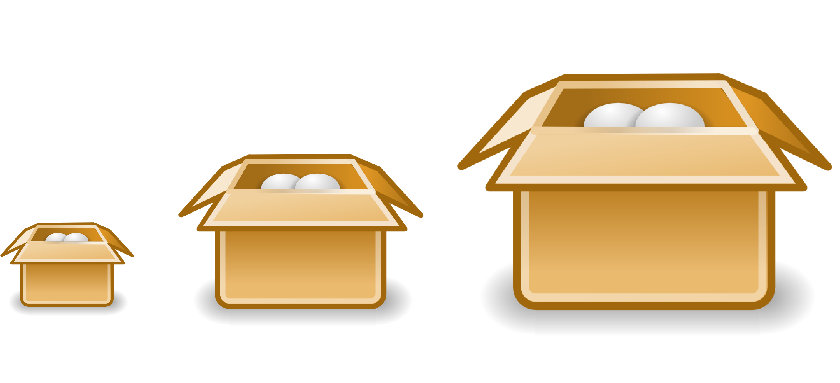
\includegraphics[width=10cm, height=5cm]{images/size.png}
      \label{fig: size}
      \caption{Tamanho das entidades.}
    \end{center}
  \end{figure}
\end{frame}

\begin{frame}
  \frametitle{Exemplos de métricas de software}
  \framesubtitle{Coesão}

  \begin{figure}
    \begin{center}
      
\includegraphics[width=10cm, height=5cm]{images/cohesion.png}
      \label{fig: cohesion}
      \caption{Pouca ou muita responsabilidade por entidade.}
    \end{center}
  \end{figure}
\end{frame}

\begin{frame}
  \frametitle{Exemplos de métricas de software}
  \framesubtitle{Acoplamento}

  \begin{figure}
    \begin{center}
      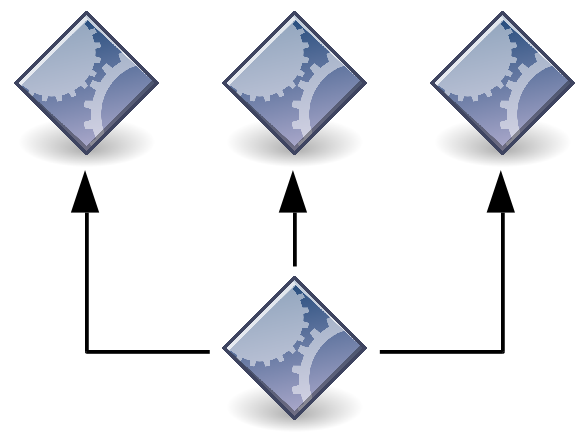
\includegraphics[width=7.5cm, height=5cm]{images/coupling.png}
      \label{fig: coupling}
      \caption{Como as entidades estão interconectadas.}
    \end{center}
  \end{figure}
\end{frame}

\begin{frame}
  \frametitle{Métricas de software}
  \framesubtitle{Problemas atuais}
  
  \begin{itemize}
    \item Não há parâmetros de comparação consolidados;
    \item Existem estudos, mas poucos dados empíricos;
    \item Ainda é dada pouca importância ao monitoramento de código.
  \end{itemize}
\end{frame}

\section{Solução}
  
\begin{frame}
  \frametitle{Proposta}
  \framesubtitle{}
  
  Encontrar conjuntos de métricas e interpretações, mantendo sua evolução no tempo, de acordo com situações específicas, através de:
  \begin{itemize}
    \item Ferramentas base para coleta das métricas\footnote{Analizo, Checkstyle, CVSAnaly etc.};
    \item Gerenciador de configurações e análise do resultado da coleta\footnote{Kalibro};
    \item Interface web para interação com a comunidade\footnote{Mezuro}.
  \end{itemize}
  

\end{frame}

  \subsection{Kalibro}
  
  \begin{frame}
    \frametitle{Kalibro}
    \framesubtitle{O que é?}
    
    \begin{figure}
      \begin{flushleft}
        
\includegraphics[width=3cm, height=1.125cm]{images/logo-kalibro.png}
        \label{fig:logo-kalibro}
      \end{flushleft}
    \end{figure}
    
    Software responsável pela coleta e análise de repositórios de acordo com métricas pré-definidas.
    \begin{itemize}
      \item Suporte a diversos controladores de versão, desde CVS até Bazaar;
      \item Aceita códigos-fonte em diversas linguagens (C, C++, Java e Python);
      \item Permite a criação de conjuntos de métricas personalizadas.
      \item Possibilita a classificação de resultados obtidos pela análise.
    \end{itemize}
  \end{frame}
  
  \subsection{Mezuro}
  
  \begin{frame}
    \frametitle{Mezuro}
    \framesubtitle{O que é?}
    
    \begin{figure}
      \begin{flushleft}
        
\includegraphics{images/logo-mezuro.png}
        \label{fig:logo-mezuro}
      \end{flushleft}
    \end{figure}
    
    \begin{itemize}
      \item Plugin para o Noosfero\footnote{Rede social livre desenvolvida pela Colivre: \url{http://noosfero.org/}}
      \item Rede de desenvolvedores de software;
      \item Visualização fácil dos resultados da análise e criação de novas configurações de métricas na Kalibro.
    \end{itemize}
  
  \end{frame}
  
  \subsubsection{Demonstração}
  
    \begin{frame}
      \frametitle{Página inicial}
      \framesubtitle{}
      
      \begin{figure}
        \begin{center}
          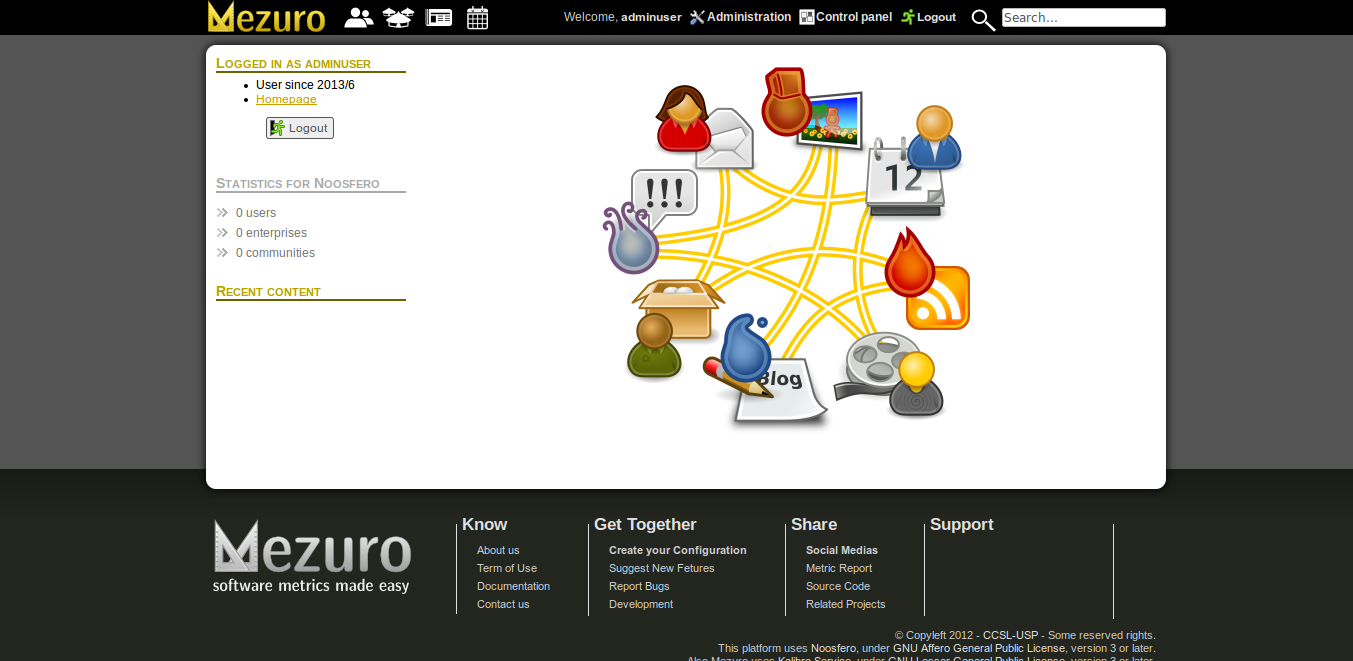
\includegraphics[width=11cm, height=6cm]{images/00-home.png}
          \label{fig:home}
        \end{center}
      \end{figure}
    
    \end{frame}
    
    \begin{frame}
      \frametitle{Lista de Comunidades}
      \framesubtitle{}
    
      \begin{figure}
        \begin{center}
          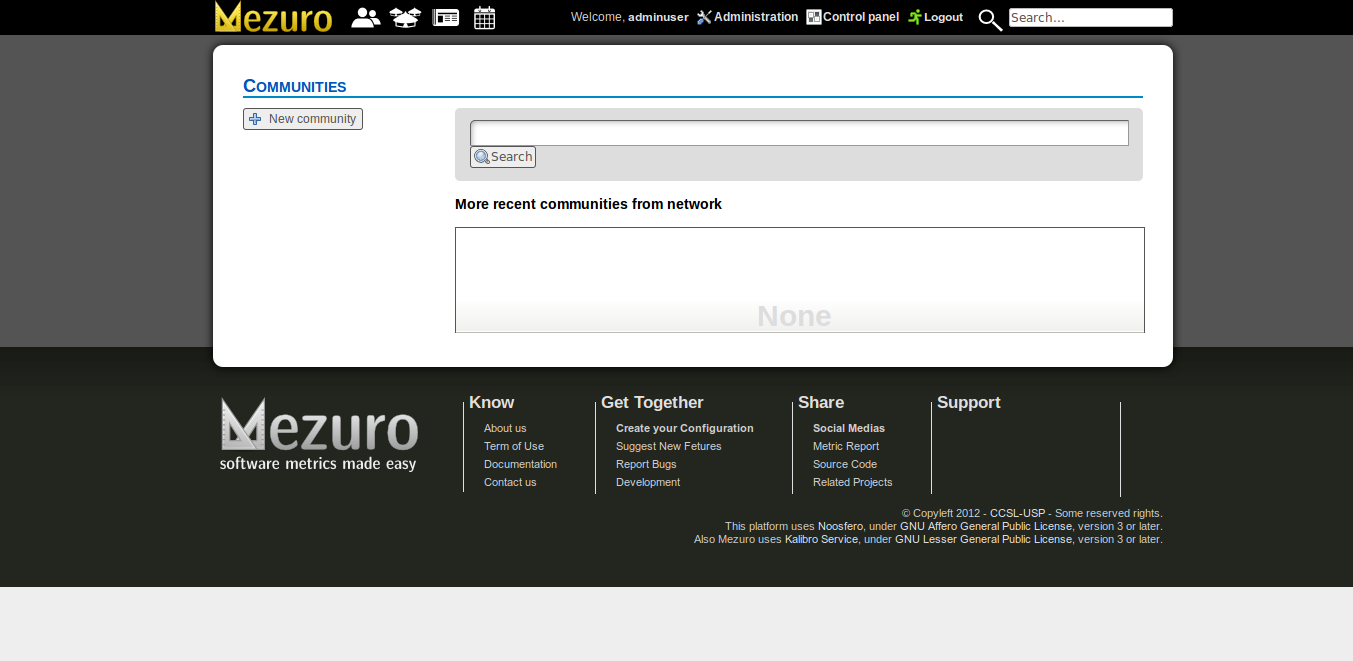
\includegraphics[width=11cm, height=6cm]{images/01-community-list.png}
          \label{fig:}
        \end{center}
      \end{figure}
    \end{frame}
    
    \begin{frame}
      \frametitle{Criação de Comunidades}
      \framesubtitle{}
    
      \begin{figure}
        \begin{center}
          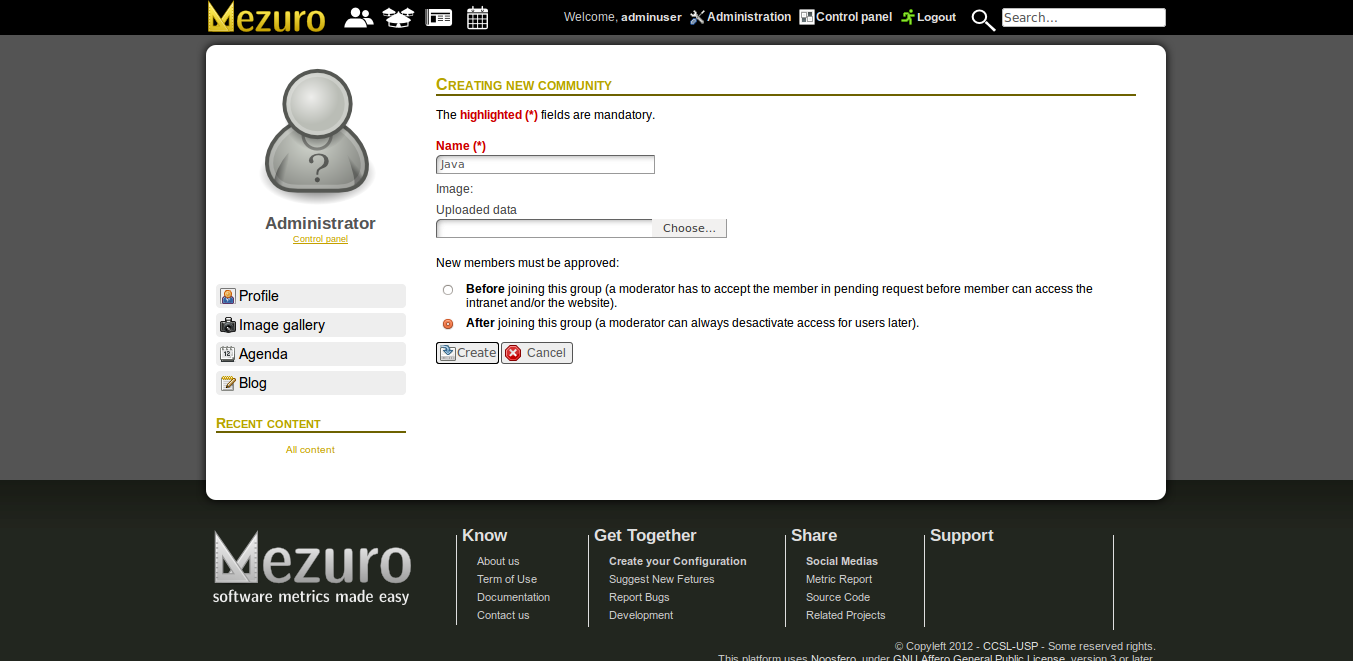
\includegraphics[width=11cm, height=6cm]{images/02-community-creation.png}
          \label{fig:}
        \end{center}
      \end{figure}
    \end{frame}
    
    \begin{frame}
      \frametitle{Comunidade Criada}
      \framesubtitle{}
    
      \begin{figure}
        \begin{center}
          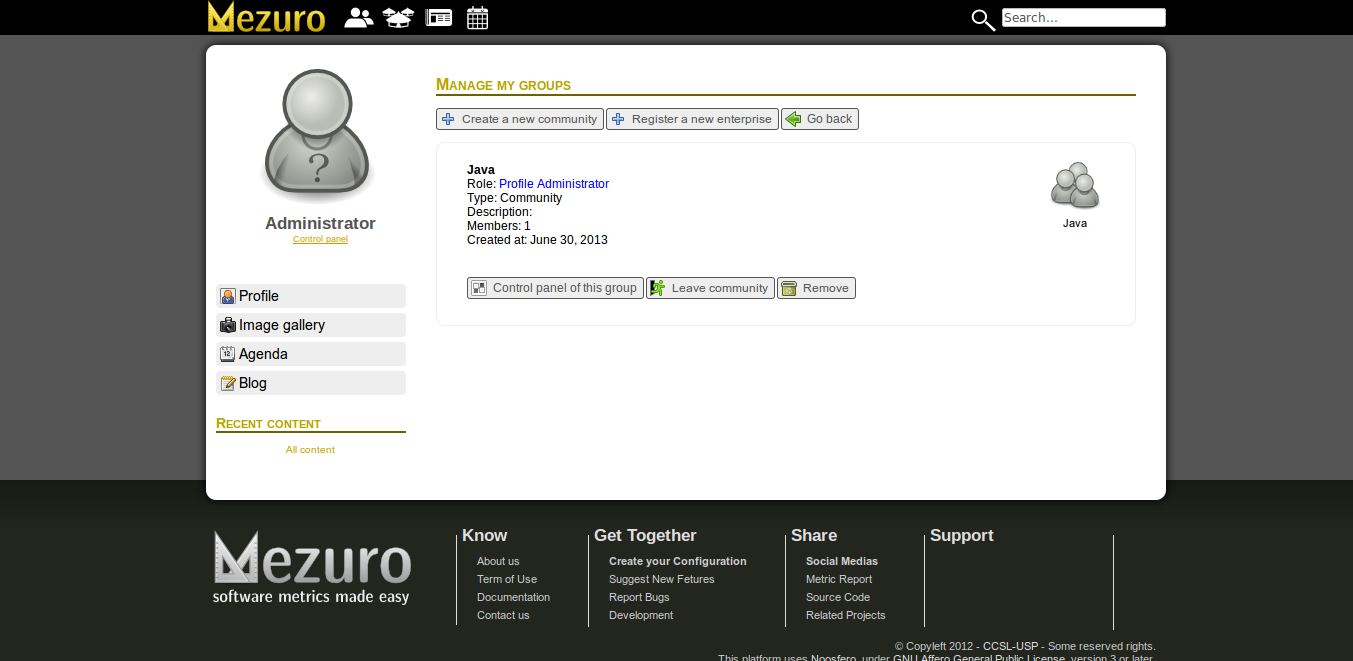
\includegraphics[width=11cm, height=6cm]{images/03-community-created.png}
          \label{fig:}
        \end{center}
      \end{figure}
    \end{frame}
    
    \begin{frame}
      \frametitle{Painel de Controle de Comunidades}
      \framesubtitle{}
    
      \begin{figure}
        \begin{center}
          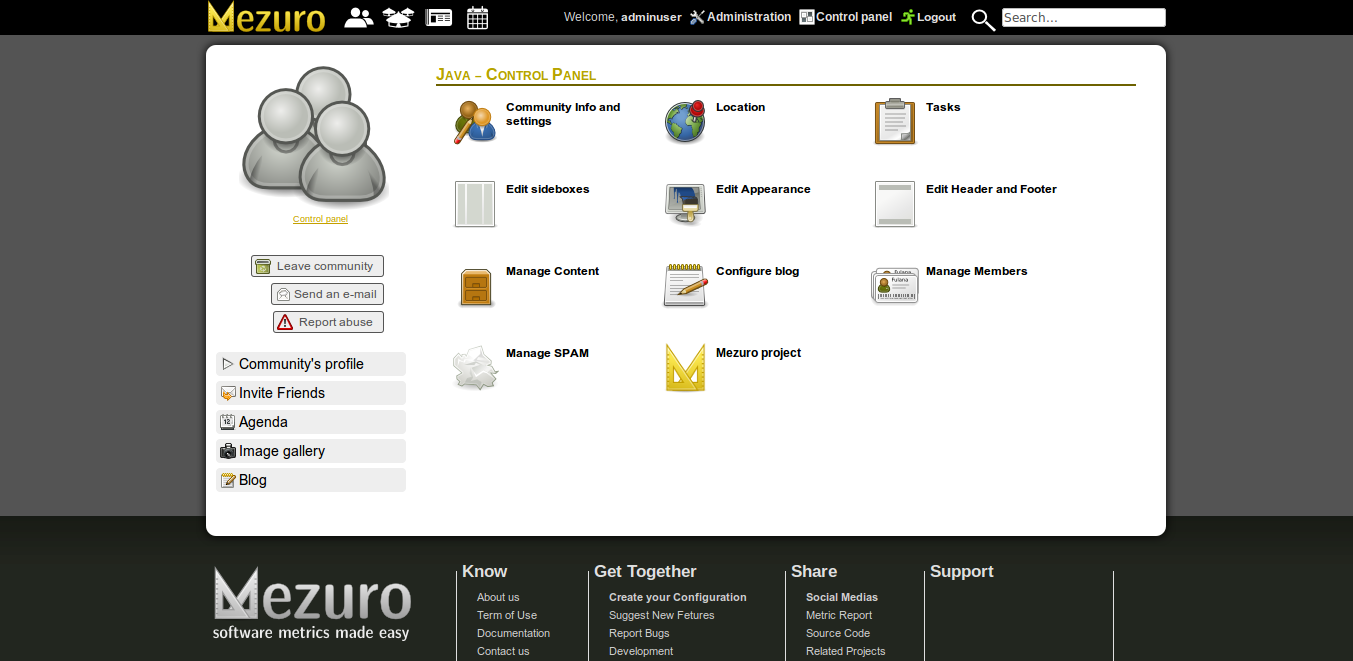
\includegraphics[width=11cm, height=6cm]{images/04-community-control-panel.png}
          \label{fig:community-control-panel}
        \end{center}
      \end{figure}
    \end{frame}
    
    \begin{frame}
      \frametitle{Criação de Projetos}
      \framesubtitle{}
    
      \begin{figure}
        \begin{center}
          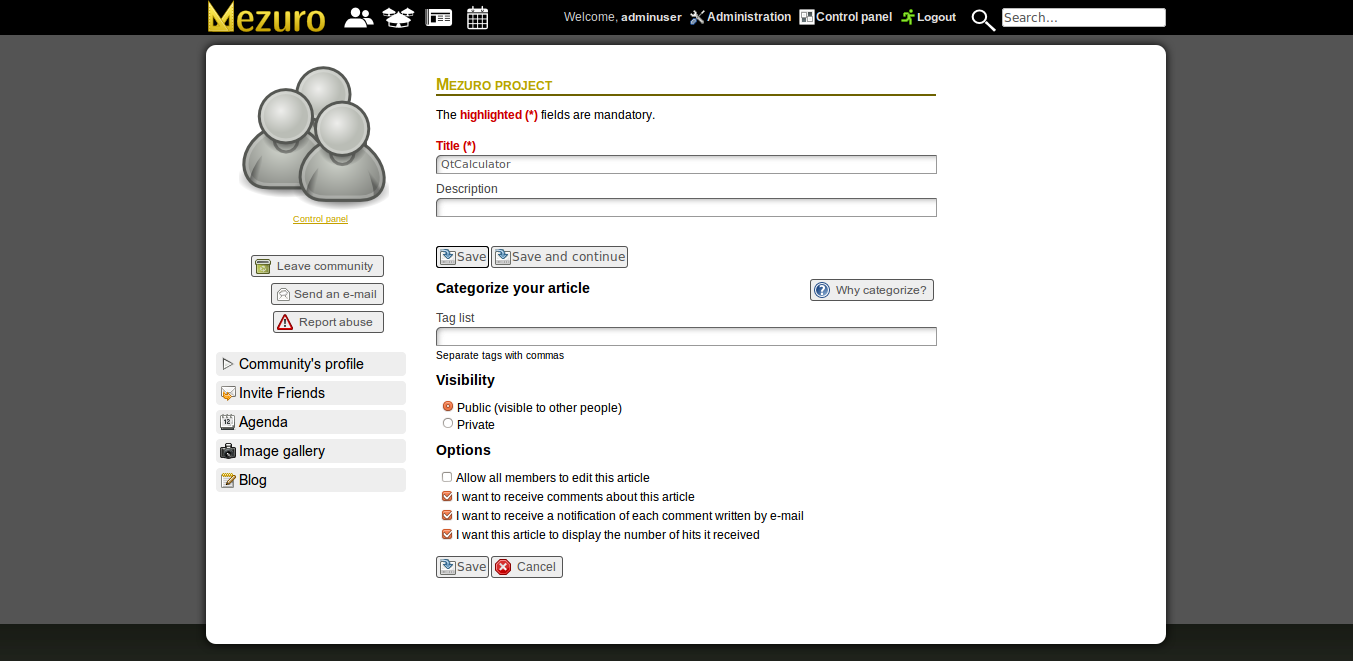
\includegraphics[width=11cm, height=6cm]{images/05-project-creation.png}
          \label{fig:project-creation}
        \end{center}
      \end{figure}
    \end{frame}
    
    \begin{frame}
      \frametitle{Projeto Criado}
      \framesubtitle{}
    
      \begin{figure}
        \begin{center}
          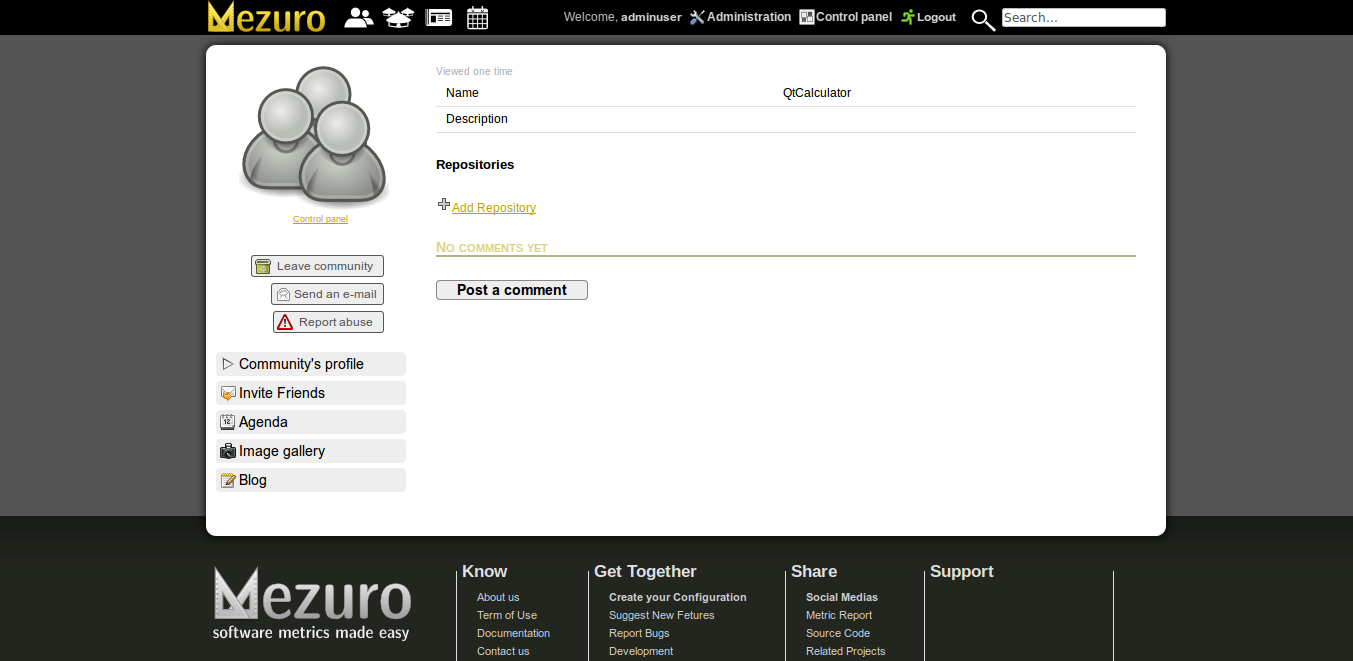
\includegraphics[width=11cm, height=6cm]{images/06-project-created.png}
          \label{fig:project-created}
        \end{center}
      \end{figure}
    \end{frame}
    
    \begin{frame}
      \frametitle{Criação de Repositório}
      \framesubtitle{}
    
      \begin{figure}
        \begin{center}
          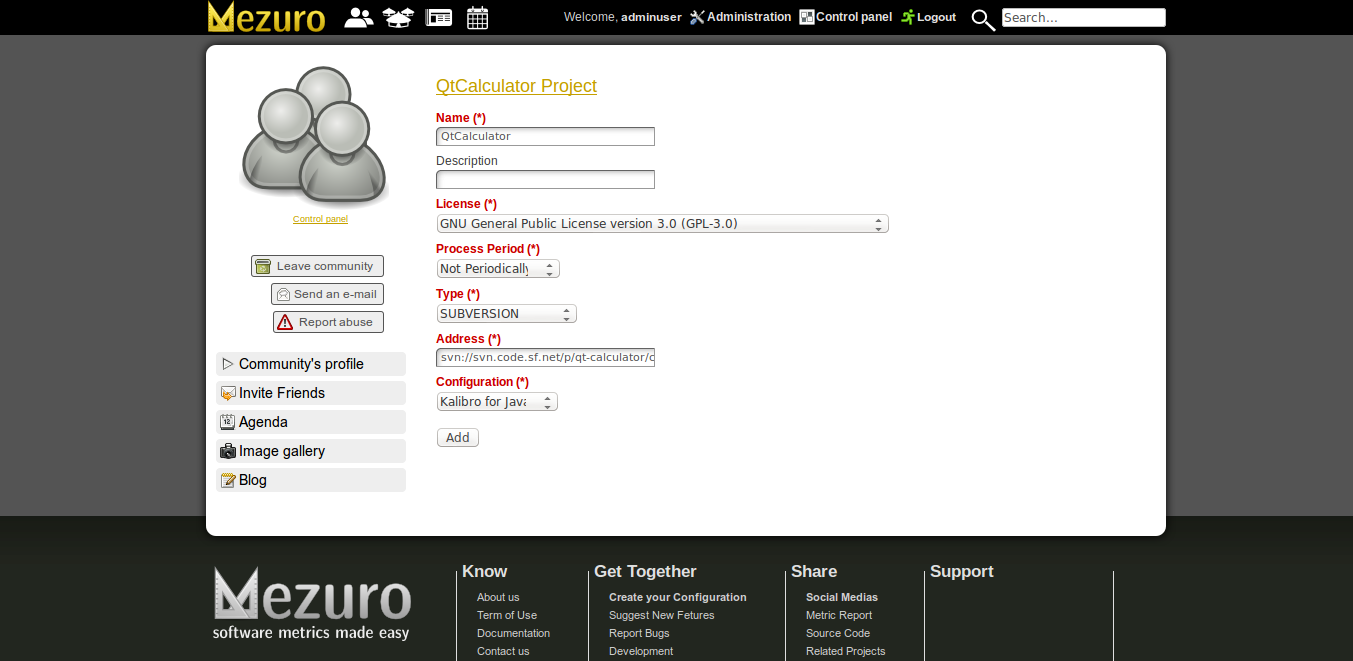
\includegraphics[width=11cm, height=6cm]{images/07-repository-creation.png}
          \label{fig:repository-creation}
        \end{center}
      \end{figure}
    \end{frame}
    
    \begin{frame}
      \frametitle{Processamento}
      \framesubtitle{}
    
      \begin{figure}
        \begin{center}
          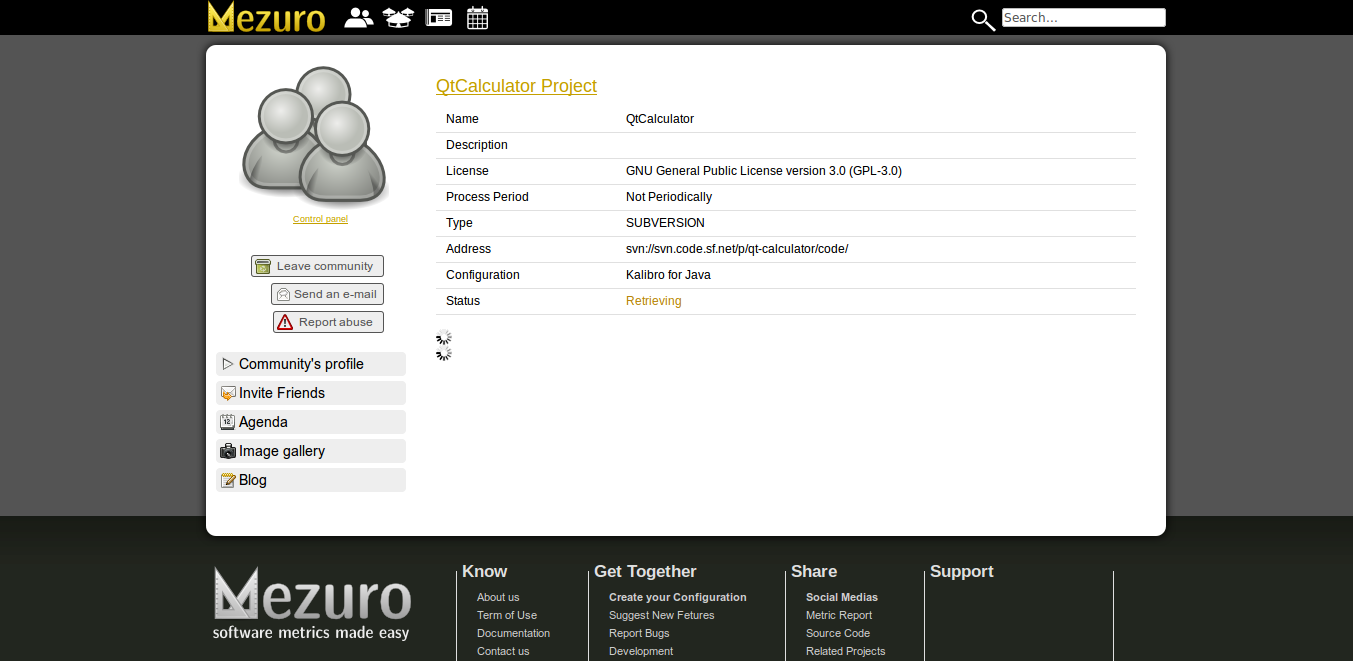
\includegraphics[width=11cm, height=6cm]{images/08-processing.png}
          \label{fig:processing}
        \end{center}
      \end{figure}
    \end{frame}
    
    \begin{frame}
      \frametitle{Estatísticas do Processamento}
      \framesubtitle{}
    
      \begin{figure}
        \begin{center}
          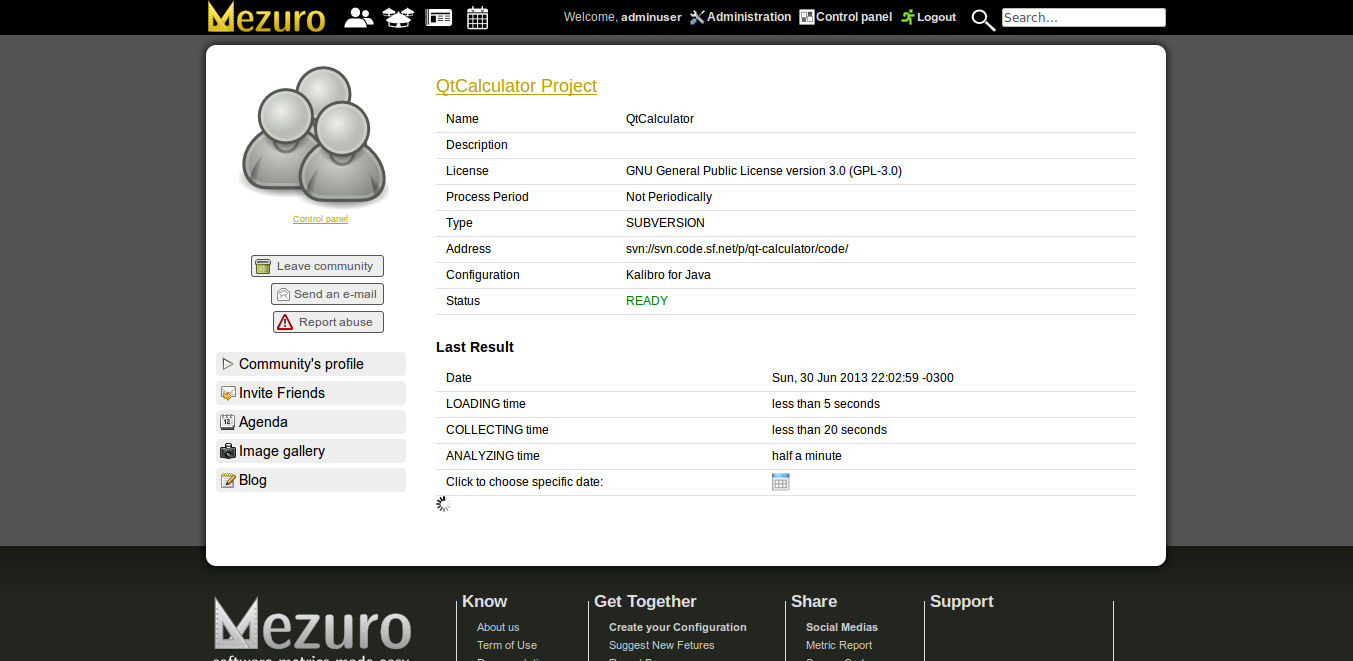
\includegraphics[width=11cm, height=6cm]{images/08-processing-stats.png}
          \label{fig:processing-stats}
        \end{center}
      \end{figure}
    \end{frame}
    
    \begin{frame}
      \frametitle{Resultados do Processamento}
      \framesubtitle{}
    
      \begin{figure}
        \begin{center}
          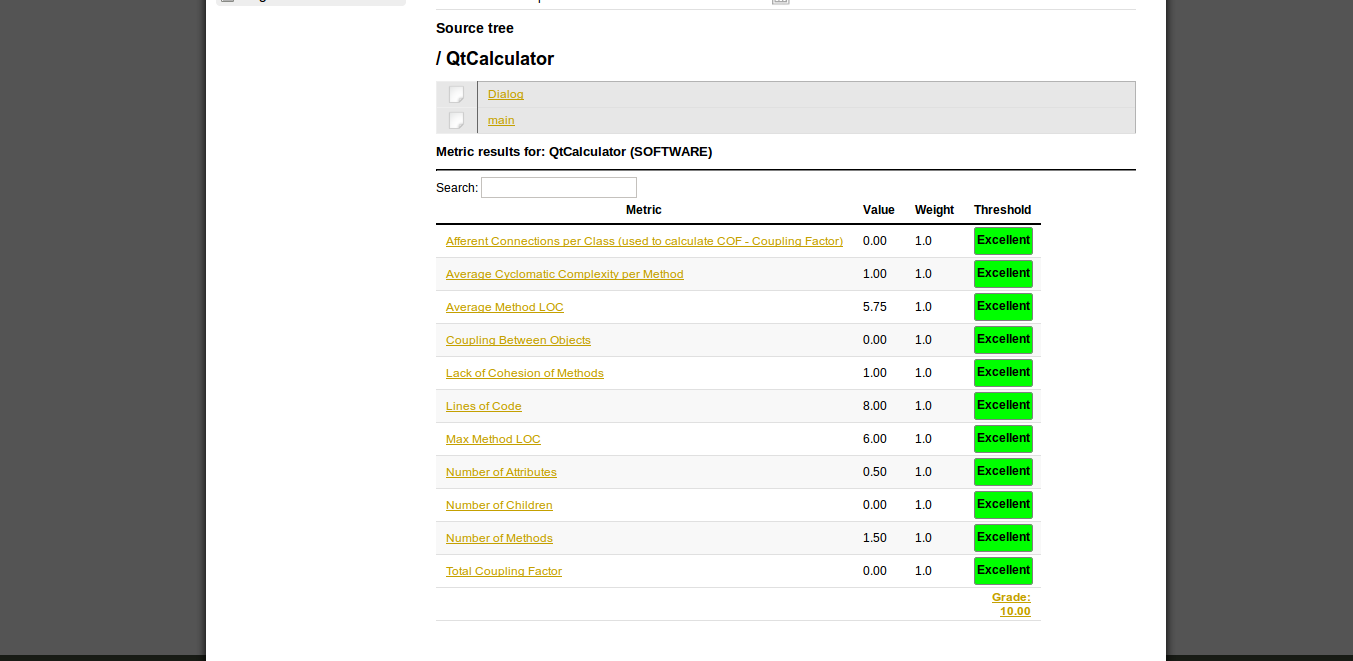
\includegraphics[width=11cm, height=6cm]{images/09-processing-results.png}
          \label{fig:processing-results}
        \end{center}
      \end{figure}
    \end{frame}
    
    \begin{frame}
      \frametitle{Gráfico de Resultados do Processamento}
      \framesubtitle{}
    
      \begin{figure}
        \begin{center}
          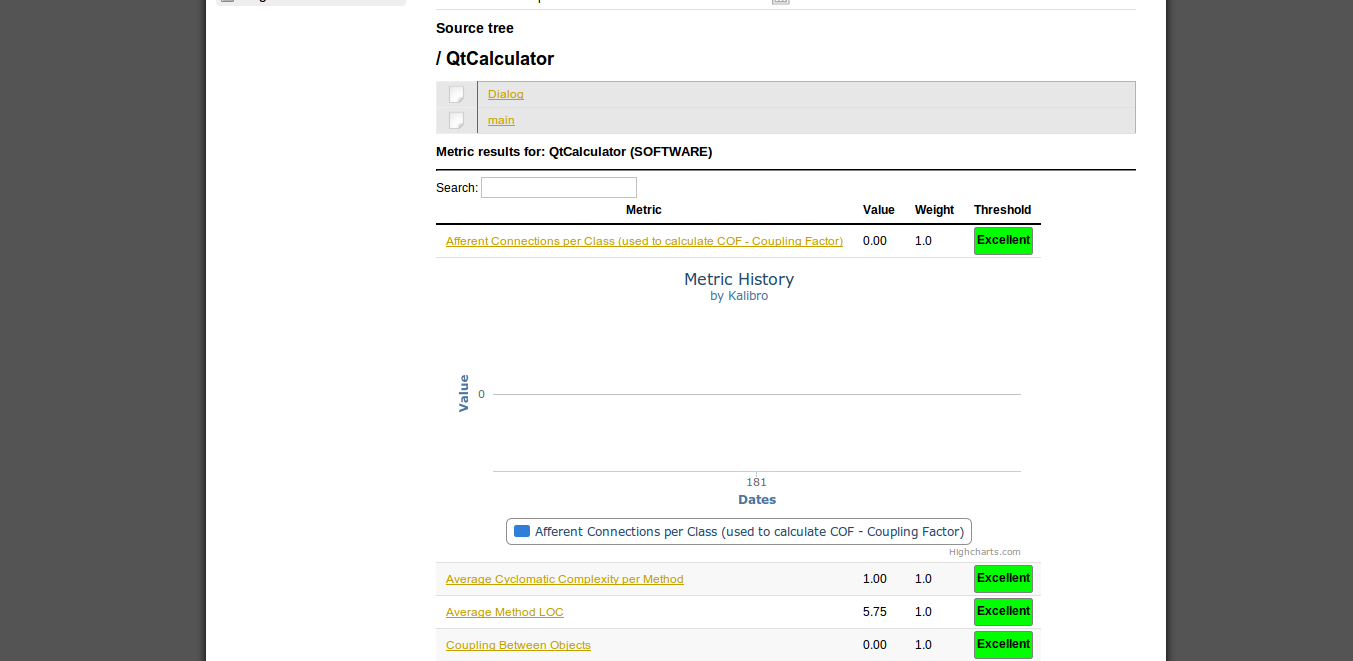
\includegraphics[width=11cm, height=6cm]{images/10-processing-results-graphic.png}
          \label{fig:processing-results-graphic}
        \end{center}
      \end{figure}
    \end{frame}
  
  \begin{frame}
    \frametitle{Conclusão}
    \framesubtitle{}
    
    \begin{itemize}
      \item Use-me: \url{http://mezuro.org};
      \item Clone-me: \url{https://github.com/mezuro/noosfero}.
    \end{itemize}
  \end{frame}
  
  \begin{frame}
    \frametitle{Próximos passos}
    \framesubtitle{Mezuro Standalone}
  
    \begin{itemize}
      \item Independente de outras plataformas;
      \item Ruby on Rails 4 + Ruby 2.0.
    \end{itemize}
    
    Clone-me: \url{https://github.com/mezuro/mezuro-standalone}.
  \end{frame}
  
    \begin{frame}
    \frametitle{Próximos passos}
    \framesubtitle{Kalibro}
  
    \begin{itemize}
      \item Gem para comunicação com a Kalibro;
      \item Análise histórica de repositórios.
    \end{itemize}
    
    Clone-me: \url{http://gitorious.org/kalibro/kalibro}.
  \end{frame}
  
  \section{Conclusão}

  \begin{frame}
    \frametitle{Agradecimentos}
    \framesubtitle{}
  
    \begin{itemize}
      \item Centro de Competência em Software Livre;
      \item Paulo Meirelles;
      \item Carlos Morais;
      \item João da Silva;
      \item Comunidade Noosfero.
    \end{itemize}
  \end{frame}

\end{document}
